\scanpage{97}

We conclude from (7) that $\ell^N$ is \uline{complete}. It suffices to prove that \deleted{\unsure{every}} \unsure{\deleted{sequence}|sequence} $(x^k)$ \deleted{in $\ell^N$} of elements $x^k\in\ell^N$, such that $\sum\lVert x^{k}\rVert_N<+\infty$, is summable in $\ell^N$. Now \deleted{it} we will have \unsure{a|:} fortiori $\sum\lVert x^k\rVert_\infty<+\infty$, so the \deleted{series} sequence will be summable in $\ell^\infty$, \inserted{to an $x\in\ell^\infty$} on the other hand we \deleted{\unsure{will have|also}} see from (7) that $x\in\ell^N$. On the other hand,

{\reversemarginpar\margin{Unnecessary, it suffices to proceed by duality : $\ell^N$ is the dual of $\ell_N$.}}

we have

\[
N\left(x-\sum_{k=1}^n x^k\right)=\deleted{\unsure{\leq|\Rightarrow}}N\left(\deleted{\unsure{x-|x}}\sum_{n+1}^\infty x^k\right)\leq\sum_{n\unsure{-|+}1}^{\unsure{n|\infty}}N(x^k),
\]

which tends to \deleted{\unsure{$\infty$|zero} \unsure{since the|for}}\inserted{$0$ for $n\to+\infty$}, since $\sum N(x^k)$ is a convergent series. It follows that we also have $\sum x^k=x$ \uline{in $\ell^N$}.

Let $\ell_N$ be the closure of $C^{(\underline N)}$ in $\ell^N$, since $\ell^N$ is complete, $\ell_N$ is identified with the completion of $C^{(\underline N)}$ for the norm $N$. It is also trivial that if $N'\leq N''$, then $\ell_{N'}\subset\ell_{N''}$, and the identity \unsure{injection|map} $\ell_{N'}\to\ell_{N''}$ has norm $\leq 1$. In particular, the spaces $\ell_N$ associated with $N_1$ and $N_\infty$ being resp. $\ell^1$ and $c_0$, we obtain

\[
\begin{array}{@{}l@{\qquad}l@{}}
(8)&\displaystyle \ell^1\subset\ell_N\subset c_0
\end{array}
\]

{\reversemarginpar\margin{
\begin{tikzpicture}[x=0.13mm,y=-0.13mm,line cap=round,line join=round]
\draw[blue!60!black,line width=0.35mm] (12,25)--(25,27)--(37,28)--(54,28)--(69,29)--(81,31)--(94,31);
\draw[blue!60!black,line width=0.3mm] (32,28)--(48,27)--(64,28)--(78,26);
\draw[blue!60!black,line width=0.3mm] (32,31)--(45,30)--(60,31)--(74,31)--(87,32);
\end{tikzpicture}}}

\uline{Proposition} We have $\ell^N\subset c_0$ unless $N$ is equivalent \unsure{to|:} $N_\infty$.

\deleted{Let us note the formula, which makes precise the \unsure{condition|properties} \unsure{above|following}}

\[
\begin{array}{@{}l@{\qquad}l@{}}
\deleted{(9)}&\displaystyle \deleted{\underline{\ell}_N=\underline{\ell}^N\cap\underline{c}_0}
\end{array}
\]

\deleted{It suffices to prove that $x\in\ell^N\cap c_0$ implies $x\in\ell_N$. \unsure{And} Indeed, we will have}\raisebox{-0.8ex}[0pt][0pt]{\makebox[0pt][r]{\begin{tikzpicture}[x=0.15cm,y=0.15cm,baseline]
\draw[line width=0.45pt] (0,0)--(0.6,0);
\fill (1.3,0) circle (0.06);
\fill (2.3,-0.02) circle (0.07);
\draw[line width=0.45pt] (3.15,-0.02)--(3.75,-0.02);
\fill (4.2,-0.02) circle (0.07);
\draw[line width=0.45pt] (5.1,-0.02)--(5.8,-0.04);
\draw[line width=0.45pt] (6.75,-0.08)--(7.65,-0.08);
\fill (8.65,-0.1) circle (0.07);
\draw[line width=0.45pt] (9.6,-0.08)--(10.2,-0.08);
\end{tikzpicture}}}

Let us note that $R^{(N)}$ is in duality with itself under the pairing $\langle x,y\rangle=\sum x_i y_i$. This makes it possible to associate to \deleted{every} a norm $N$ on $R^{(N)}$, the \uline{polar norm}, denoted $N'$, defined by

\[
\begin{array}{@{}l@{\qquad}l@{}}
(9)&\displaystyle N^\circ(y')=\underset{N(\unsure{y|x})\leq 1}{\operatorname{Sup}}\,|\langle x,y'\rangle|
\end{array}
\]

{\reversemarginpar\margin{Moreover, \unsure{then|clearly} \unsure{we have} $(N^\circ)^\circ=N$, we can verify it .... \deleted{\unsure{we are reduced} \unsure{to|to the|from} \illegible{1}}}}

If $N$ is a Schatten norm, we verify
{\reversemarginpar\margin{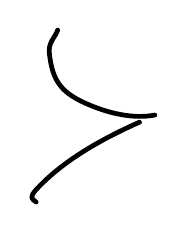
\begin{tikzpicture}[x=0.13mm,y=-0.13mm,line cap=round,line join=round]
\draw[line width=0.6mm] (45,21) .. controls (43,28) and (35,33) .. (37,45) .. controls (40,69) and (47,81) .. (71,92) .. controls (95,103) and (120,108) .. (140,104);
\draw[line width=0.6mm] (125,111) .. controls (91,126) and (50,148) .. (23,178) .. controls (18,184) and (19,186) .. (24,189);
\end{tikzpicture}}}
trivially that $N^\circ$ is a Schatten norm, and We \unsure{will say|say} that \deleted{the dual of $\ell_N$ is identified with $\ell^{N'}$, the accou\unsure{p|pl} \unsure{being|ment} $\sum x_i x_i'$ is \unsure{absolutely} summable, and that} \inserted{if $u\in\ell_N$, $u'\in\ell^{N^\circ}$, then \deleted{\unsure{we have the}}}

{\reversemarginpar\margin{98}}
